\documentclass[french]{article}
\usepackage[utf8]{inputenc}
\usepackage[T1]{fontenc}
\usepackage{lmodern}
\usepackage[a4paper]{geometry}
\usepackage{babel}
\usepackage{graphicx}

\title{On a flaw in the CUSUM algorithm under the gaussian hypothesis}
\author{Clément Bonvoisin, Pierre Ludmann}
\date{06/06/2014}

\begin{document}
\maketitle

\section{The theory behind the flaw}
The following document shows a case in which the CUSUM algorithm does not detect what is, to the eye - and according to the mathematical definition -, a change point in a signal.
\linebreak
\linebreak
Let's start with a few reminders. A discrete signal $(X_t)_{t \in \{1..n\}}$ is considered as a finite sequence of random variables.
\\ \\
A change point is a time $t_0$ such that :
\begin{itemize}
	\item $\forall t < t_0, X_t$ follows a distribution $p_0$
	\item $\forall t \geq t_0, X_t$ follows a distribution $p_1$
\end{itemize}
It is implicit here that $p_0 \ne p_1$. This definition naturally extends to the case of a number $\kappa$ of change points in the signal.
\\ \\
The CUSUM algorithm was introduced by E.S. Page in 1954 to try to solve the problem of online detection of change points. It can be adapted to an offline point of view.
\\ \\
To establish the formulas on which our algorithm is based, we make the hypothesis that our signals are generated by gaussian distributions; we thus have 2 parameters for our distributions : the mean $\mu$ and the standard deviation $\sigma$. These are the only parameters that our algorithm takes into account.
\\ \\
We can now see that a potential flaw of our implementation of the CUSUM algorithm is that two distributions can have the same mean and variance, and yet not be the same. We present here the example of a Beta and a Gamma distribution.
\\ \\
As a reminder, a Beta distribution has two parameters, $\alpha$ and $\beta$, with :
\begin{itemize}
	\item[mean] : $\frac{\alpha}{\alpha + \beta}$
	\item[variance] : $\frac{\alpha \beta}{(\alpha + \beta)^2(\alpha + \beta + 1)}$
\end{itemize}
A Gamma distribution also has two parameters, usually called $k$ and $\theta$, with :
\begin{itemize}
	\item[mean] : $k \theta$
	\item[variance] : $k \theta ^2$
\end{itemize}
Here, we want the means and variances to be the same. It is easy to show that this happens iff :
\begin{equation}
	\left\lbrace 
	\begin{array}{l}
	 
	\theta = \frac{\beta}{(\alpha + \beta)(\alpha + \beta + 1)}\\
	 
	k = \frac{\alpha(\alpha + \beta + 1)}{\beta}
	 
	\end{array}\right.
	\label{eq1}
\end{equation}

\section{Application : let's make the CUSUM fail}
Using MATLAB, we create a signal X with :
\begin{itemize}
	\item From 0 to 10,000 : $X_t$ follows a distribution $\beta (1,2)$
	\item From 10,001 to 20,000 : $X_t$ follows a distribution $\Gamma (2, 1/6)$
\end{itemize}

We can easily see that this fits the equation \ref{eq1}. Fig. \ref{flaw} shows the signal X.

\begin{figure}[h]
	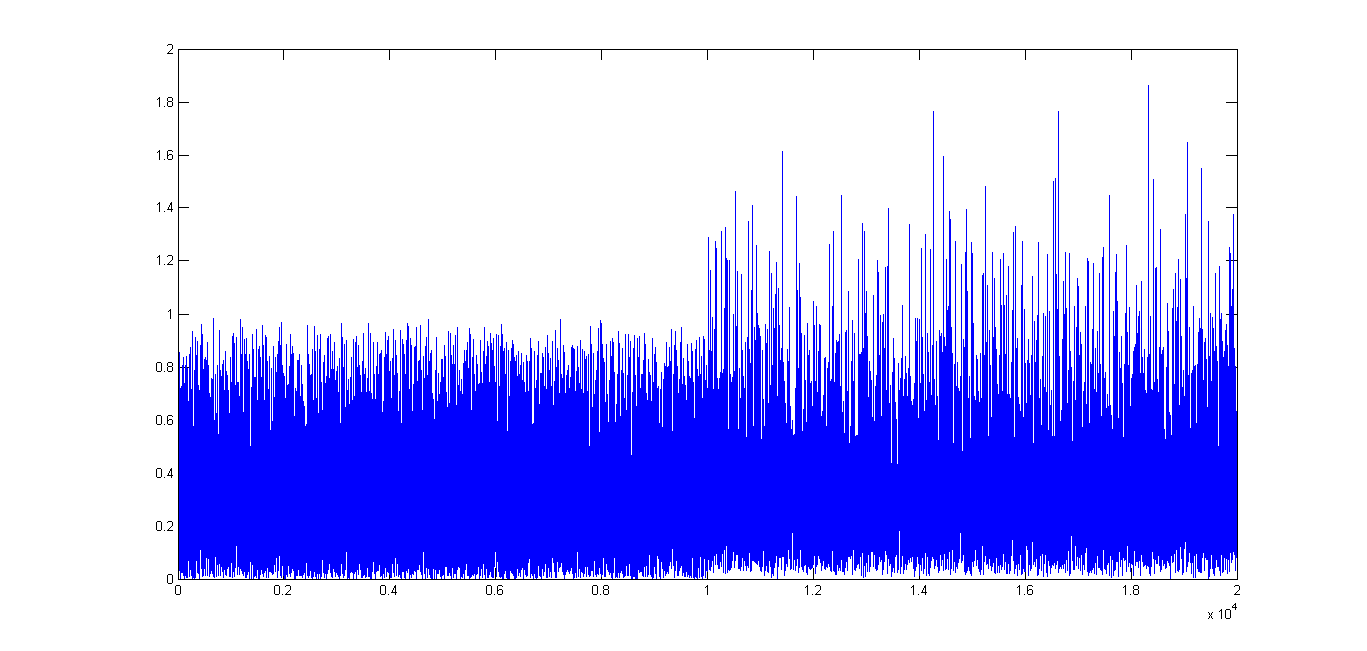
\includegraphics[scale=0.4]{flawsignal.png}
	\caption{From 0 to 10,000 : $\beta (1,2)$ ; from 10,001 to 20,000 : $\Gamma (2, 1/6)$}
	\label{flaw}
\end{figure}

We can now apply the CUSUM algorithm as we implemented it, in order to make it fail. The theoretical change point is 10,001 ; yet, the CUSUM algorithm's answer is :
\begin{itemize}
	\item based on mean : 7
	\item based on standard deviation : 19,863
	\item based on both : 19,863
\end{itemize}

The following is what was typed in MATLAB to get these answers :

\begin{verbatim}
>> pdf1 = makedist('Beta', 'a', 1, 'b', 2);
>> pdf2 = makedist('Gamma', 'a', 2, 'b', 1/6);
>> X = [random(pdf1, 10000, 1) ; random(pdf2, 10000, 1)];
>> [time, value] = dikt_cusum_lin(X, {'mean'}, 1)
time =
     7
value =
    3.1925
>> [time, value] = dikt_cusum_lin(X, {'std'}, 1)
time =
       19863
value =
    4.2608
>> [time, value] = dikt_cusum_lin(X, {'both'}, 1)
time =
       19863
value =
    5.8029
>> [mean(X(1:10000)) , mean(X(10001:20000))]
ans =
    0.3352    0.3311
>> [std(X(1:10000)) , std(X(10001:20000))]
ans =
    0.2362    0.2350
\end{verbatim}

\section{Conclusion on this example}
This example shows that the CUSUM algorithm, as implemented under the hypothesis that the given signals are issued from a gaussian distribution, focuses on change points that include a change in mean and/or variance, and that we can create signals with a visible change point (here, at 10,000) and no change in mean and/or variance, and thus make the CUSUM algorithm fail - if we don't respect the gaussian hypothesis.
\\ \\
Let us note that this failure is not inherent to the CUSUM algorithm as described by E.S. Page, but to the hypothesis that our signals are always generated by gaussian distributions. This forces the signal to have all its moments of order $\geq 2$ equal to 0, and thus the CUSUM can only focus on the mean and variance of the signal.

\section{Failed segmentation of a Cognac-G signal : practical case}
Our internship focuses on signals recorded from an experience (a patient walks, makes a U-turn, and then walks back). A consequence of the above discussion is that in order to be sure that we can use the CUSUM algorithm to find the change points in these signals, they must be generated by a gaussian distribution.
\\ \\
This is, of course, a rather natural hypothesis, given the properties of the gaussian distribution. Yet, as shown in the figures below, the CUSUM algorithm fails on certain signals.
\\ \\
The following figures show the detection of eight change points in one of those signals (AKR-Zou-YO-2-Xsens). Each figure represents the detection of a new change point.

\begin{figure}[h]
	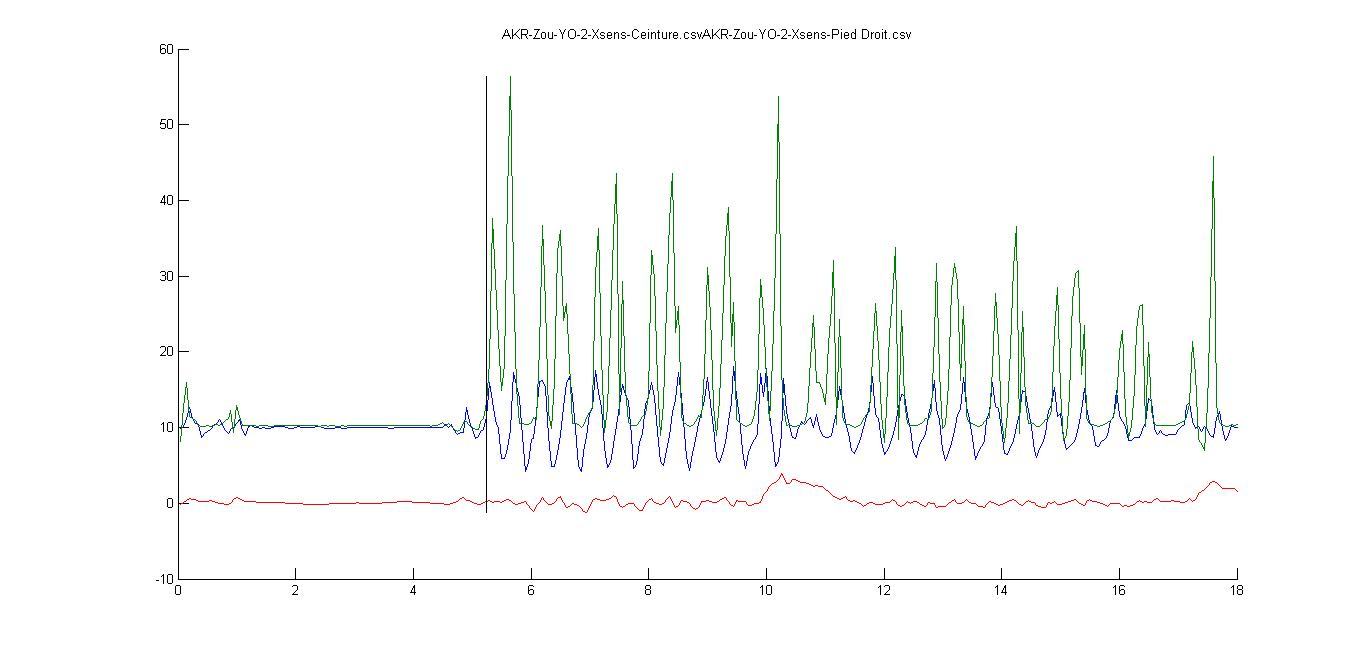
\includegraphics[scale=0.3]{seg1.jpg}
	\caption{First change point}
	\label{1ststep}
\end{figure}

\begin{figure}[h]
	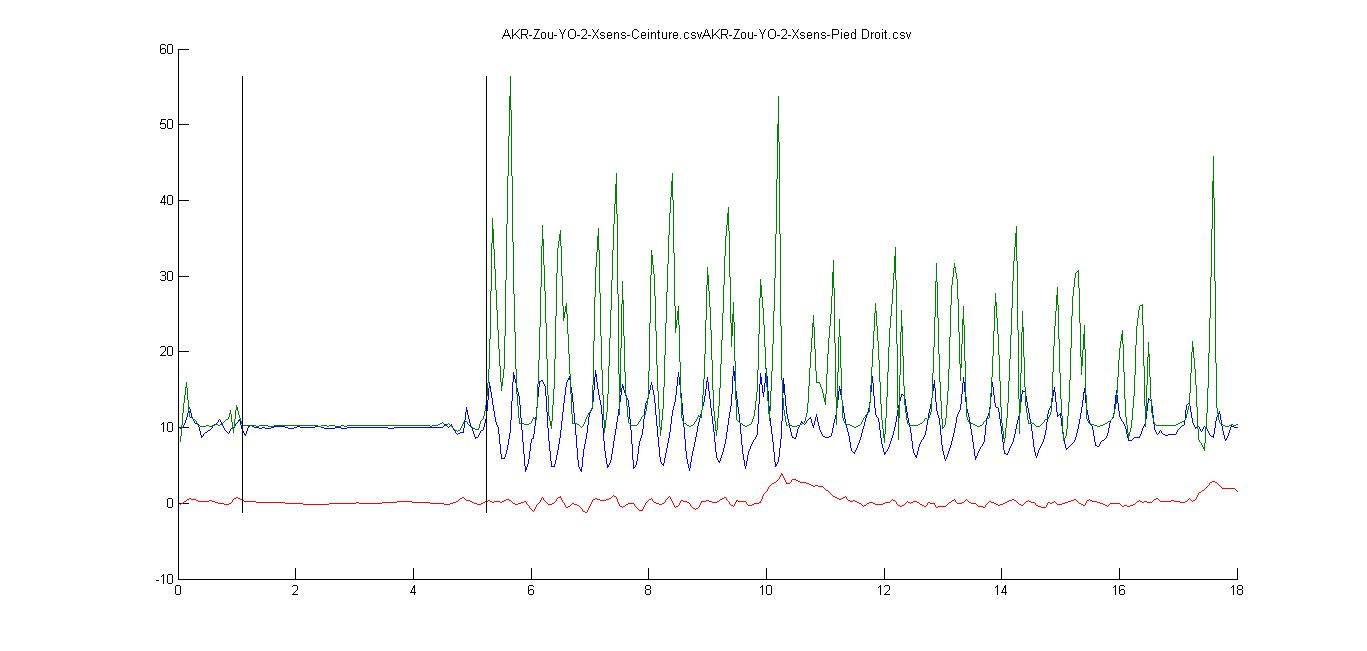
\includegraphics[scale=0.3]{seg2.jpg}
	\caption{Second change point}
\end{figure}

\begin{figure}[h]
	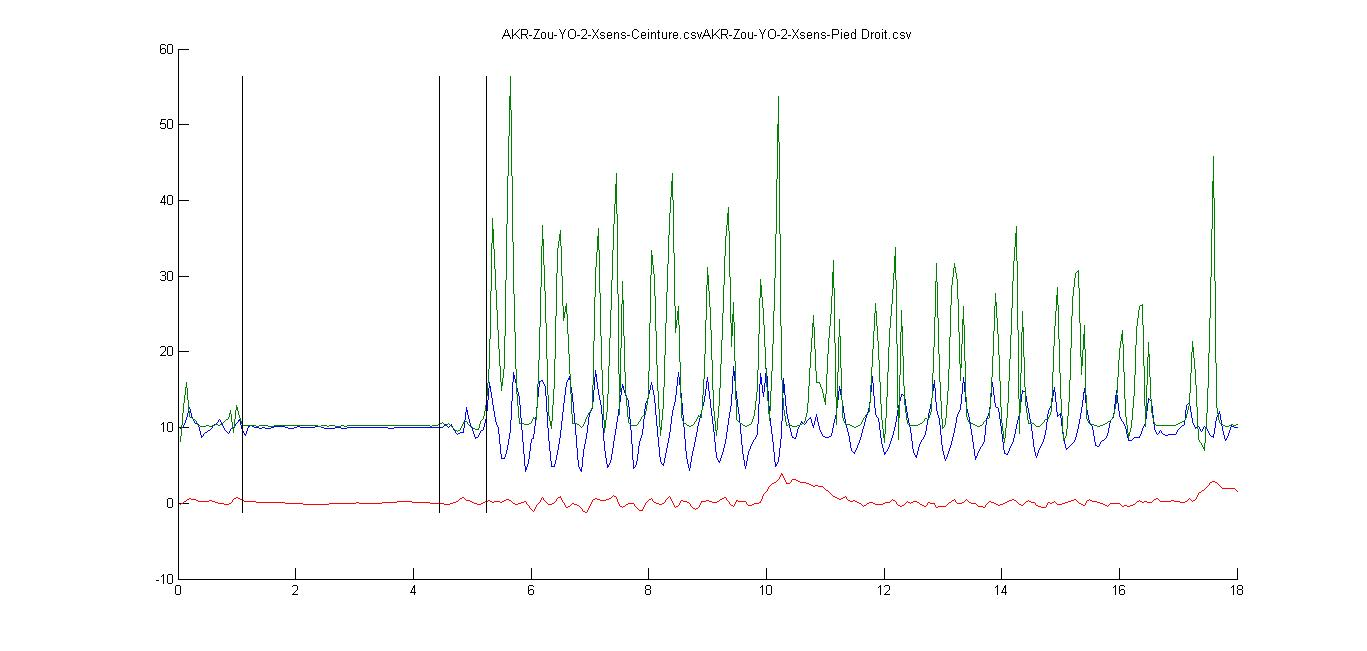
\includegraphics[scale=0.3]{seg3.jpg}
	\caption{Third change point}
\end{figure}

\begin{figure}[h]
	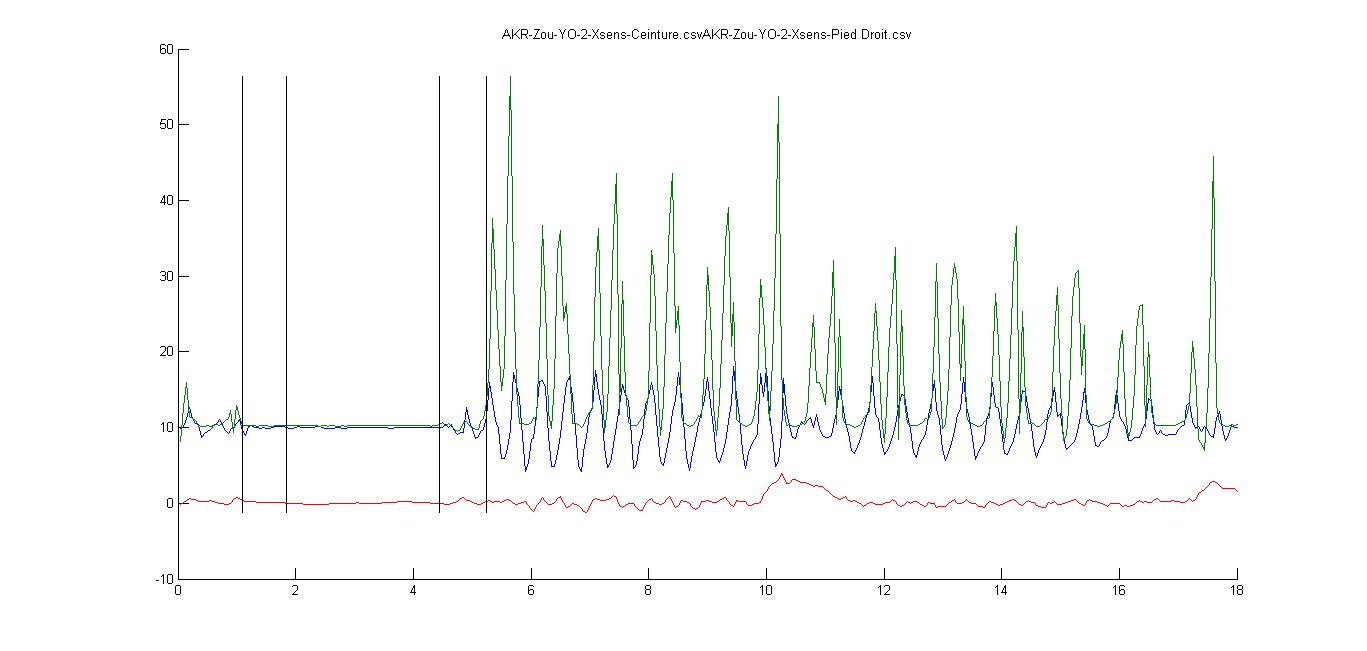
\includegraphics[scale=0.3]{seg4.jpg}
	\caption{Fourth change point}
\end{figure}

\begin{figure}[h]
	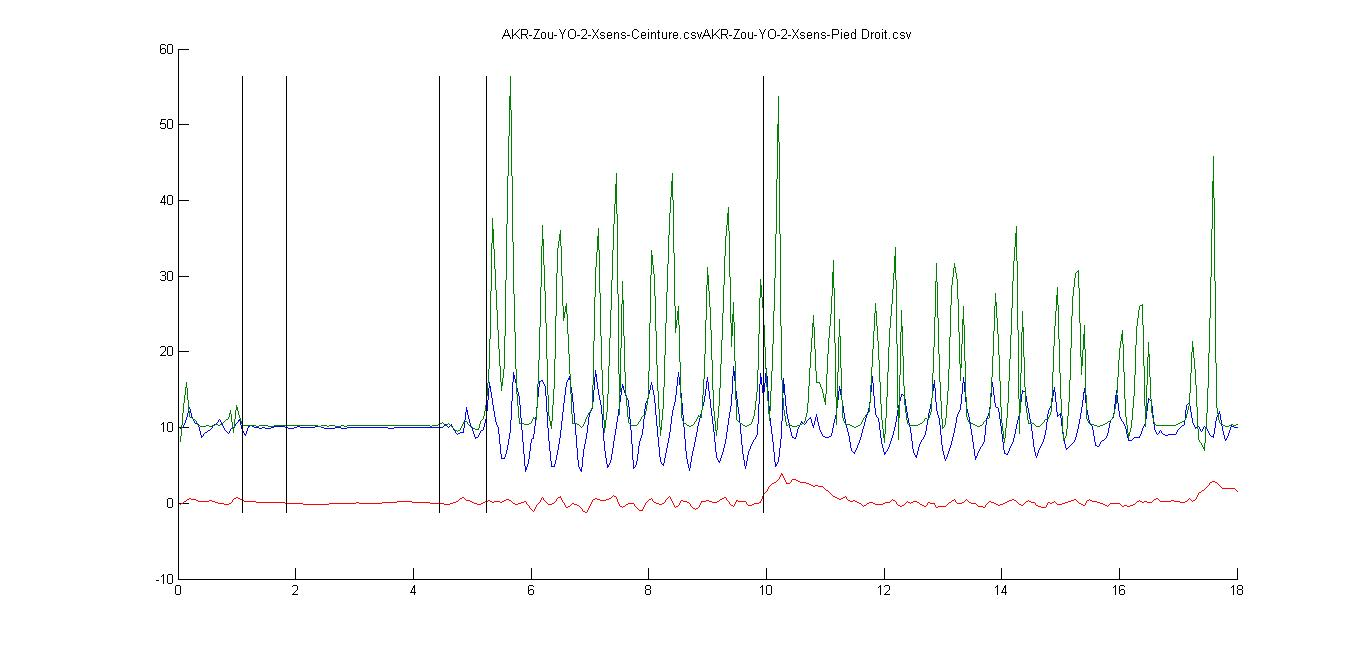
\includegraphics[scale=0.3]{seg5.jpg}
	\caption{Fifth change point}
\end{figure}

\begin{figure}[h]
	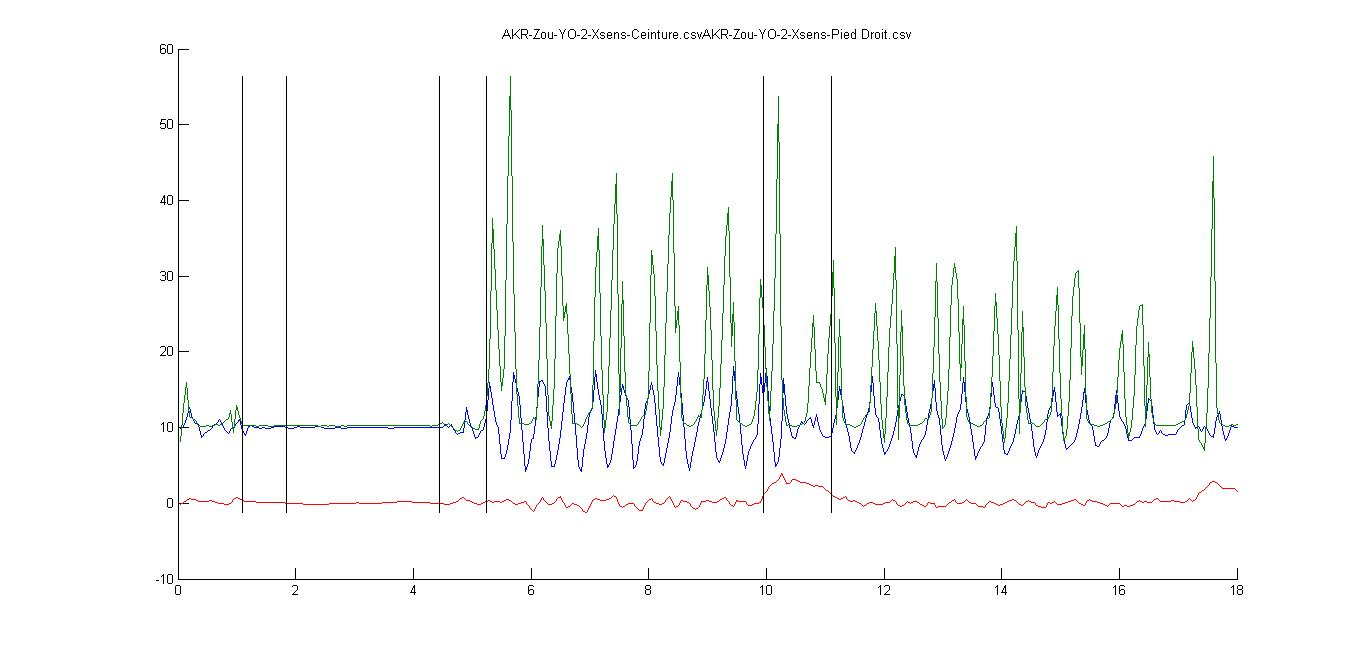
\includegraphics[scale=0.3]{seg6.jpg}
	\caption{Sixth change point}
\end{figure}

\begin{figure}[h]
	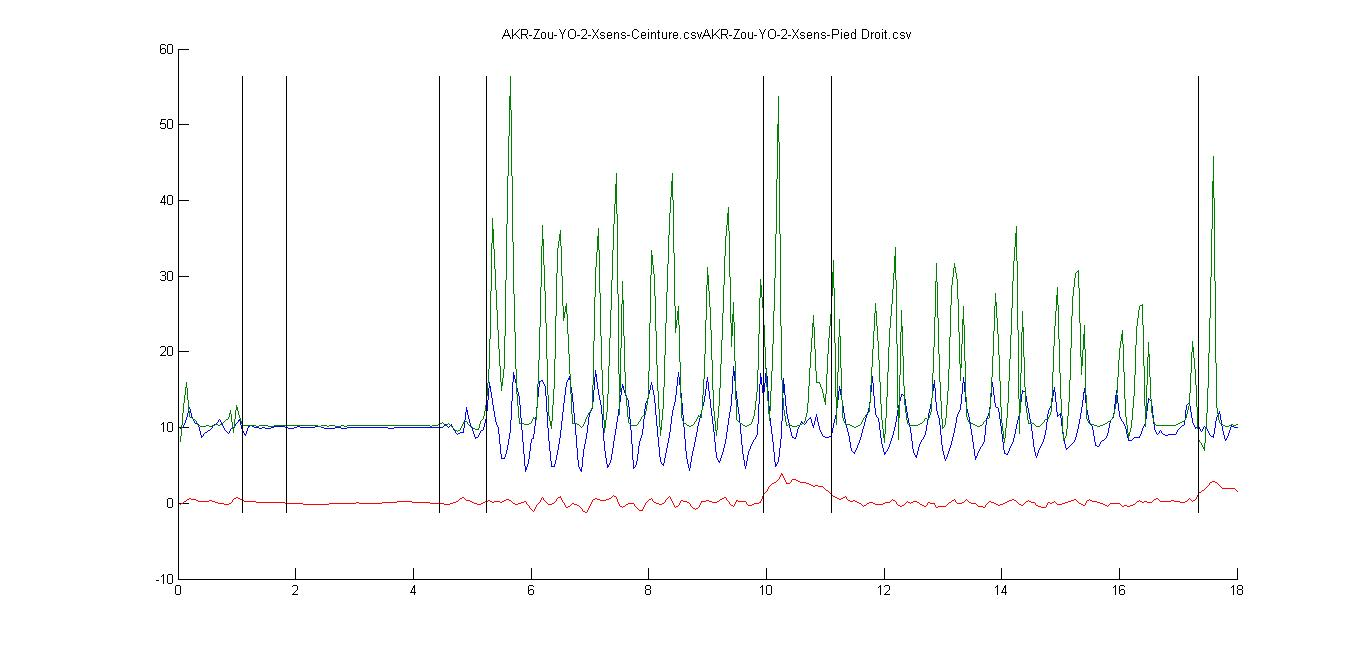
\includegraphics[scale=0.3]{seg7.jpg}
	\caption{Seventh change point}
\end{figure}

\begin{figure}[h]
	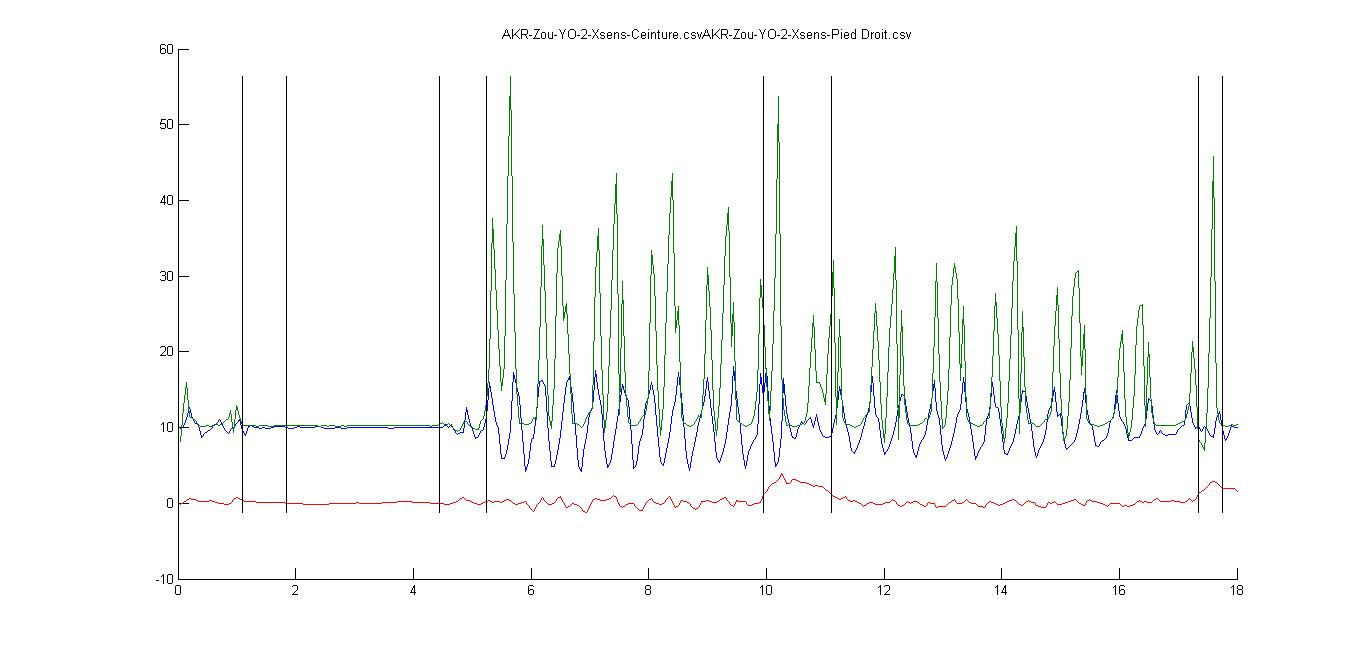
\includegraphics[scale=0.3]{seg8.jpg}
	\caption{Eigth change point}
\end{figure}

The first change point detected by the CUSUM algorithm makes sense : it is the beginning of the walk ; the second change point is the end of a problem at the beginning of the signal. In between the third and first change points is the phase during which the patient makes its first step. But then, the fourth change point seems to be kind of irrelevant, as opposed to the fifth (which is the beginning of the U-turn).
\\ \\
Further explorations show that when trying to detect the fifth change point, the distribution that generates the signal isn't really gaussian, as shown in the following figures.

\begin{figure}[h]
	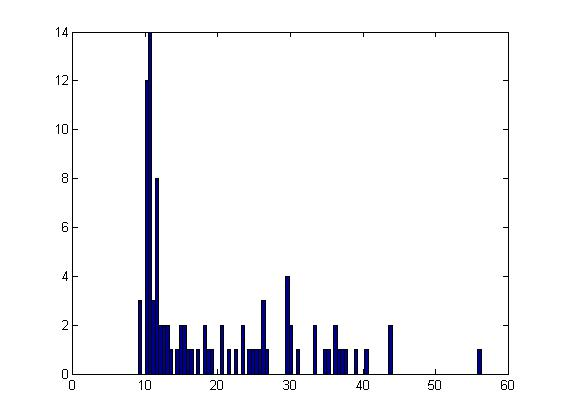
\includegraphics[scale=0.7]{hist1_1-foot.jpg}
	\caption{Before the fifth change point - foot}
\end{figure}

\begin{figure}[h]
	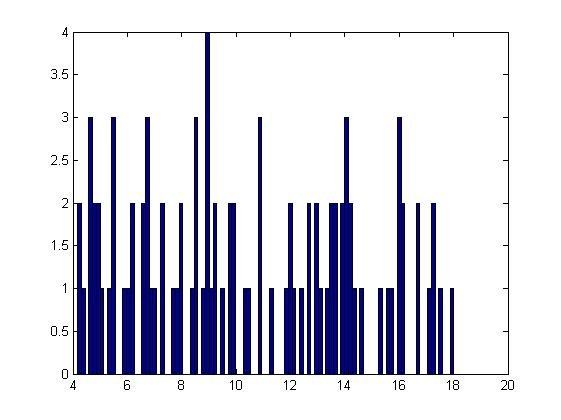
\includegraphics[scale=0.7]{hist2_1-back.jpg}
	\caption{Before the fifth change point - back}
\end{figure}

\begin{figure}[h]
	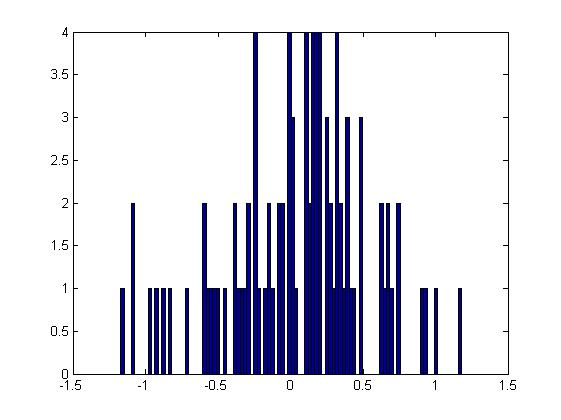
\includegraphics[scale=0.7]{hist3_1-gyr.jpg}
	\caption{Before the fifth change point - gyration}
\end{figure}

\begin{figure}[h]
	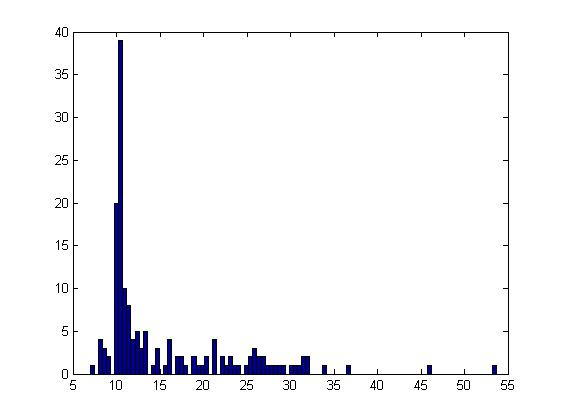
\includegraphics[scale=0.7]{hist1_2-foot.jpg}
	\caption{After the fifth change point - foot}
\end{figure}

\begin{figure}[h]
	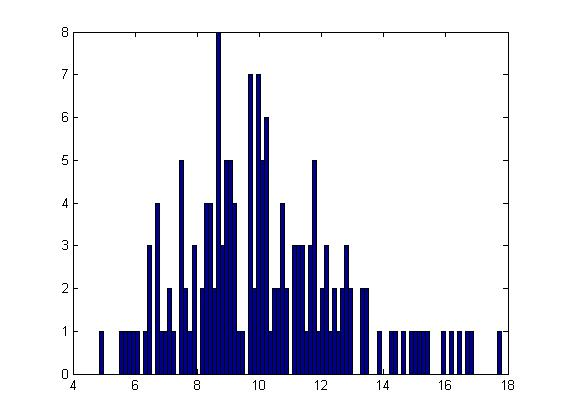
\includegraphics[scale=0.7]{hist2_2-back.jpg}
	\caption{After the fifth change point - back}
\end{figure}

\begin{figure}[h]
	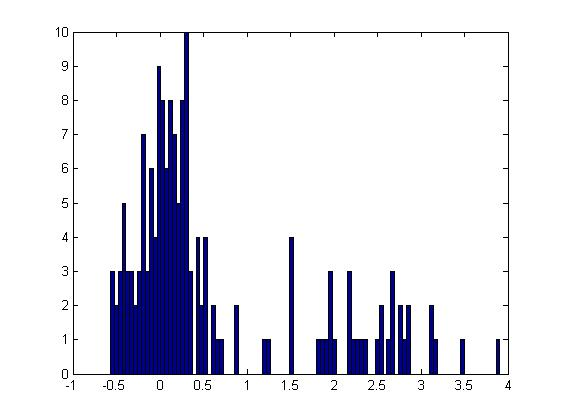
\includegraphics[scale=0.7]{hist3_2-gyr.jpg}
	\caption{After the fifth change point - gyration}
\end{figure}

\end{document}
